\documentclass[../main.tex]{subfiles}
\graphicspath{{\subfix{../img/}}}
\begin{document}

\newpage
\section{Simulator}

Der Simulator dient dazu, die Funktionalität der Software des autonomen Fahrzeugs zu testen, bevor der physische Prototyp gebaut wird.\\

\subsection{Spezifikation}

In diesem Abschnitt wird definiert, was der Simulator genau leisten soll. Die Anforderungen stammen aus der Aufgabenstellung sowie dem gewählten Fahrzeugkonzept.

\begin{table}[htbp!]
    \centering
    \begin{tabularx}{\textwidth}{| l | X | l |}
        \hline
        \textbf{Nr.} & \textbf{Spezifikation} & \textbf{Priorität} \\ \hline
        1. & Es wird (ohne Beachtung der Hindernisse) immer der schnellste Weg ins Ziel gefunden. & Hoch \\ \hline
        2. & Entfernte Linien werden nicht befahren. & Hoch \\ \hline
        3. & Linien mit Hindernissen werden erkannt und nur befahren, falls ein Umweg länger dauert. & Hoch \\ \hline
        4. & Neue Informationen können während der Fahrt aufgenommen und entsprechende Strategie-Anpassungen dazu vorgenommen werden. & Hoch \\ \hline
        5. & Das Ziel kann konfiguriert werden (A, B oder C) & Hoch \\ \hline
        6. & Es gibt ein User Interface, welches den befahrenen Graphen aufzeigt. & Hoch \\ \hline
        6.1 & Im User Interface werden Pylonen, Hindernisse und entfernte Linien aufgezeigt & Mittel \\ \hline
        7. & Kommandos, die an die Hardware geschickt werden sollen, werden ausgegeben. & Mittel \\ \hline
        8. & Der Simulator analysiert den Graphen anhand von Bildern. & Tief \\ \hline
    \end{tabularx}
\end{table}

\newpage
\subsection{Morphologischer Kasten}

\newcolumntype{Y}{>{\centering\arraybackslash}X}

\begin{table}[htbp!]
    \centering
    \begin{tabularx}{\textwidth}{| X | Y | Y | Y |}
        \hline

        \rowcolor{LightGray}
        \textbf{Funktion} & \textbf{Option 1} & \textbf{Option 2} & \textbf{Option 3} \\ \hline
        
        \textbf{User Interface} &     
        Terminal \newline
        
\includegraphics[width=2.5cm]{img/simulation/morphologischer-kasten/terminal.png}
        &
        \cellcolor{LightGreen}
        Einfaches GUI \newline
        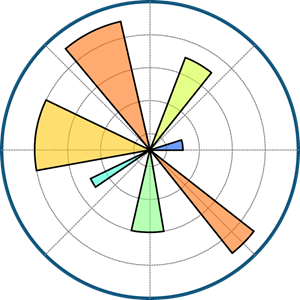
\includegraphics[width=2.5cm]{img/simulation/morphologischer-kasten/simple-gui.png}
        &
        Unreal Engine \newline
        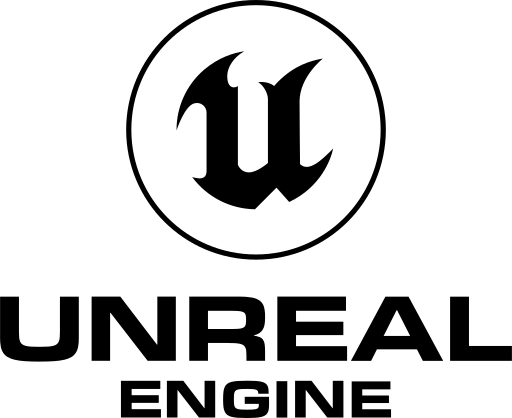
\includegraphics[width=2.5cm]{img/simulation/morphologischer-kasten/unreal-engine-logo.png}
        \\ \hline
        
        \textbf{Wegfindungs-Algorithmus}  &
        \cellcolor{LightGreen}
        Externe Bibliothek &
        Eigene Implementation &
        \\ \hline
        
        \textbf{Programmiersprache}      &
        \cellcolor{LightGreen}
        Python \newline
        
\includegraphics[width=2.5cm]{img/simulation/morphologischer-kasten/python.png} 
        &
        JavaScript \newline
        
\includegraphics[width=2.5cm]{img/simulation/morphologischer-kasten/javascript.png}
        &
        Java \newline
        
\includegraphics[width=2.5cm]{img/simulation/morphologischer-kasten/java.png}
        \\ \hline
        
        \textbf{Informationen \newline einlesen}  &     
        Bilder mit Objekterkennung \newline
        
\includegraphics[width=2.5cm]{img/simulation/morphologischer-kasten/ai-logo.jpg}
        &
        \cellcolor{LightGreen}
        Konfigurationsdatei \newline
        
\includegraphics[width=2.5cm]{img/simulation/morphologischer-kasten/yaml.png}
        &
        \\ \hline
        
        \textbf{Hindernis \newline Bewältigung}   &     
        Immer umfahren \newline
        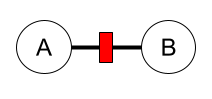
\includegraphics[width=3cm]{img/simulation/morphologischer-kasten/hindernis-umfahren.png}
        &
        Keine spezielle Behandlung \newline
        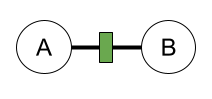
\includegraphics[width=3cm]{img/simulation/morphologischer-kasten/hindernis-ignoriert.png}
        &
        \cellcolor{LightGreen}
        Gewicht hinzufügen\newline
        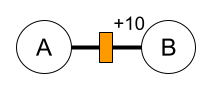
\includegraphics[width=3cm]{img/simulation/morphologischer-kasten/hindernis-gewicht.png}
        \\ \hline
    \end{tabularx}
    \caption{Morphologischer Kasten - Simulator}
\end{table}

Der Lösungsansatz des Morphologischen Kastens ist darauf ausgelegt, einen simplen Simulator zu erstellen, welcher trotzdem viele Anforderungen an die Wegfindung abdecken kann.

\subsubsection{User Interface}

Obwohl ebenfalls eine virtuelle Umgebung mit der Unreal Engine und dem Pfadfinder-Model existiert, ist der Aufwand zu gross, diese an den Simulator anzubinden. Die Ausgabe in einem Terminal hingegen ist zu minimal. Deshalb wird das User Interface mit einem einfachen GUI umgesetzt. 

\subsubsection{Wegfindungs-Algorithmus}

Die Umsetzung des Wegfindungs-Algorithmus kann entweder eigenständig oder mithilfe einer externen Bibliothek erfolgen. Da zahlreiche etablierte Bibliotheken für die Graphentheorie verfügbar sind, erscheint eine eigenständige Implementierung nicht sinnvoll. Dies führt zwar zu einer geringeren Flexibilität, reduziert jedoch die Fehleranfälligkeit erheblich.

\subsubsection{Programmiersprache}

Für die Wahl der Programmiersprache wurden Python, JavaScript und Java in Betracht gezogen. Java ist im Informatik-Studium weit verbreitet und wird für zahlreiche Projekte eingesetzt. JavaScript bietet die Möglichkeit, grafische Darstellungen unkompliziert über eine Webseite zu realisieren. Python zeichnet sich durch seine einfache Handhabung aus und wird häufig im Bereich der Künstlichen Intelligenz verwendet, was für die Software des autonomen Roboters wichtig ist.

Python wurde als Programmiersprache gewählt, da innerhalb des Teams umfassendes Know-how vorhanden ist. Darüber hinaus stellt die Bibliothek NetworkX\footnote{https://networkx.org} eine leistungsstarke Lösung für die Arbeit mit Graphen bereit, die optimal für die Anforderungen des Projekts geeignet ist.

\subsubsection{Informationen einlesen}

Damit die Software die Hindernisse auf dem Graphen kennt, müssen entsprechende Informationen eingelesen werden können. Idealerweise erfolgt dies ähnlich wie in der Realität, durch die Auswertung von Bildern mittels Objekterkennung. Um den Simulator jedoch möglichst schnell einsatzfähig zu machen, wird stattdessen eine Konfigurationsdatei verwendet, die die notwendigen Informationen bereitstellt.

Die Konfigurationsdatei ermöglicht eine einfache Anpassung der Szenarien und erlaubt dadurch das effiziente Testen verschiedener Konstellationen. Diese Herangehensweise beschleunigt die Entwicklungsphase und sorgt für Flexibilität beim Simulieren diverser Bedingungen.

\subsubsection{Hindernis Bewältigung}

Der Simulator soll aufzeigen, wie Hindernisse auf der Strecke behandelt werden.
Dabei wird berücksichtigt, dass Hindernisse unter bestimmten Bedingungen nicht immer umfahren werden können, beispielsweise wenn sämtliche alternativen Wege blockiert sind. Daher stellt die Option `Immer umfahren` keine sinnvolle Strategie dar.

Das Ignorieren von Hindernissen ist ebenfalls suboptimal, da gleich lange Pfade ohne Hindernisse effizienter befahren werden können. Um diesem Problem zu begegnen, wird die Strategie `Gewicht hinzufügen` angewendet. Mit dieser Methode kann flexibel entschieden werden, wie stark ein Hindernis die Wahl eines Pfades beeinflusst. Die Gewichtung erlaubt es, Hindernisse dynamisch in die Berechnung einzubeziehen, ohne zwingend alle Alternativen auszuschliessen.

\subsection{Konzept}

Im Optimalfall würde der Simulator die gesamte Hardware des autonomen Fahrzeugs nachbilden. Dadurch könnte die Fahrzeugsoftware direkt im Simulator getestet werden, ohne Anpassungen vornehmen zu müssen. Diese Herangehensweise würde eine nahtlose Integration zwischen Softwareentwicklung und Simulation ermöglichen. Allerdings ist die vollständige Simulation der Hardware mit erheblichem Aufwand verbunden und übersteigt den Rahmen des Simulators.

Der Simulator wird so konzipiert, dass er anhand einer vorgegebenen Konfiguration den optimalen Weg zum Ziel findet. Diese Konfiguration beinhaltet:
\begin{itemize}
    \item Das Ziel: A, B oder C.
    \item Die Gewichtung für das Befahren von Linien mit einem Hindernis.
    \item Informationen die erst beim Befahren eines neuen Wegpunktes freigeschalten werden:
     \begin{itemize}
        \item Wegpunkte mit einem Pylon 
        \item Entfernte Linien
        \item Erkannte Hindernisse
   \end{itemize}
\end{itemize}


Damit die Simulation weiss, auf welchen Wegpunkten bzw. Linien sich Hindernisse befinden, wird jeder Wegpunkt beschriftet:

\imagewidth{img/simulation/labeled-graph.png}{Beschrifteter Graph}{10cm}

Die Konfiguration wird in einer \acrshort{yaml}-Datei abgespeichert und sieht wie folgt aus.

\begin{minted}[fontsize=\small]{yaml}
end: B
weight: 3
S:
  cones: [E]
  obstacles: 
    - [S, F] 
  removed:
    - [E, A]
D:
  obstacles:
    - [D, A]
  removed:
    - [D, B]
\end{minted}

In der Beispielkonfiguration wird das Ziel \textbf{B} definiert. Hindernisse auf Linien erhalten eine \textbf{dreifache Gewichtung} im Vergleich zu normalen Linien. 

Zu Beginn der Simulation, am Knoten \textbf{S}, erhält die Software folgende Informationen:
\begin{itemize}
    \item Auf dem \textbf{Knoten E} befindet sich eine Pylone.
    \item Auf der \textbf{Kante S-F} befindet sich ein Hindernis.
    \item Die \textbf{Kante E-A} ist nicht vorhanden.
\end{itemize}

Zusätzlich wird beim Befahren vom Wegpunkt \textbf{D} folgendes festgestellt:
\begin{itemize}
    \item Auf der \textbf{Kante D-A} befindet sich ein Hindernis.
    \item Die \textbf{Kante D-B} ist nicht vorhanden.
\end{itemize}

Diese Informationen werden genutzt, um den Graphen dynamisch zu aktualisieren und die optimalen Routen basierend auf den aktuellen Bedingungen neu zu berechnen.


\subsection{Umsetzung}

TODO(Gian): Kapitel vervollständigen

Der Simulator 
\imagewidth{img/simulation/simulator.png}{Screenshot des Simulators in Aktion}{10cm}


Verwendete Bibliotheken:

\begin{itemize}
    \item NetworkX
    \item Matplotlib
\end{itemize}

\end{document}